\documentclass[12pt]{article}
\usepackage{amsmath}
\usepackage{color}
\usepackage{enumitem}
\usepackage[margin=1in]{geometry}
\usepackage{parskip}
\usepackage{siunitx}
\usepackage{tikz}
\usepackage{ulsy}
\usetikzlibrary{calc,decorations.pathmorphing,matrix}
\newcommand{\hilight}[1]{\colorbox{yellow}{#1}}
\begin{document}

\begin{centering}
\subsection*{MSci 261 Engineering Economics: Financial Management for Engineers}
\subsubsection*{Spring 2014}
\subsubsection*{Assignment 1}
\end{centering}

\begin{itemize}
\item Print out the assignment and write down your answer in the blank place leave for you.
\item Write down the steps and highlight your final answer.
\item You need to submit this assignment by 5:00 pm on May 23 (Friday) TAs will pick it up exactly at 5:00 pm, and yours won’t be collected if you are late. You get zero for late submission.
\item Only 5 questions will be marked. The 5 questions will be picked randomly.
\item The marked assignment will be returned to you as quickly as possible. See Learn for any announcement of assignment pickup.
\end{itemize}

First Name: Kevin\\
Last Name: Carruthers\\
Student ID:\ 20463098

\vspace{40pt}

Total Mark: \line(1,0){100}

\begin{center}
\begin{tabular}{| p{3cm}| p{3cm}| p{3cm}| p{3cm}|}
  \hline
  Question 1 & & Question 6  &  \\[1cm]
  \hline
  Question 2 & & Question 7  &  \\[1cm]
  \hline
  Question 3 & & Question 8  &  \\[1cm]
  \hline
  Question 4 & & Question 10 &  \\[1cm]
  \hline
  Question 5 & &  &  \\[1cm]
\hline
\end{tabular}
\end{center}
\newpage

\begin{enumerate}[label=\textbf{Q\arabic*}]
\item For your bank account with an interest rate of 10\% compounded daily, if you deposit \$5,000 now, how much will you have after one year?
  \begin{align*}
  F &= P{(1+i)}^n\\
  &= 5000{\bigg(1 + \frac{0.1}{365}\bigg)}^{365}\\
  &= 5525.78
  \end{align*}
  I will have \hilight{\$5,525.78} after one year.
\item Violeta has paid mortgage payments of \$2,000 per month for 10 years and paid off the mortgage. What is the original mortgage loan amount, given an interest rate of 12\%?
  \begin{align*}
  P &= A\bigg(\frac{{(1+i)}^{n} - 1}{i\times {(1+i)}^n}\bigg)\\
  &= 2000\bigg(\frac{{(1+\frac{.12}{12})}^{120} - 1}{0.01\times {(1+\frac{.12}{12})}^{120}}\bigg)\\
  &= 2000\bigg(\frac{{(1.01)}^{120} - 1}{0.01\times {(1.01)}^{120}}\bigg)\\
  &= 139401.04
  \end{align*}
  The original loan amount was \hilight{\$139,401.04}.
\item You want to buy a \$2,000 laptop, but you now have only \$500. The seller gives you an introductory offer in which you pay \$500 now and \$2200 two years later. What monthly interest rate is the seller charging?
  \begin{align*}
  F &= P{(1+i)}^n\\
  \frac{F}{P} &= {(1+i)}^n\\
  \sqrt[n]{\frac{F}{P}} &= 1+i\\
  \sqrt[n]{\frac{F}{P}} - 1 &= i\\
  i &= \sqrt[2\times 12]{\frac{2200}{1500}} - 1\\
  i &= \sqrt[24]{\frac{22}{15}} - 1\\
  i &= 0.0161
  \end{align*}
  The monthly interest was \hilight{1.61\%}
\item A local car dealer has an ad in the newspaper for a new car as follows: ``For a \$30,000 car we will give you \$1,000 cash back and 0\% interest for 36 months''. (In other words you only pay \$29,000 for the car.) If banks charge an annual interest rate on loans of 12\% compounded monthly, what is the present worth of the car?
  \begin{align*}
  P &= A\bigg(\frac{{(1+i)}^n - 1}{i{(1+i)}^n}\bigg)\\
  &= \frac{29000}{36}\bigg(\frac{{(1+\frac{.12}{12})}^{36} - 1}{\frac{.12}{12}{(1+\frac{.12}{12})}^{36}}\bigg)\\
  &= 24253.40
  \end{align*}
  The present worth of the car is \hilight{\$24,253.40}.
\item A \$25,000 bond, which carries a 16\% coupon rate with quarterly payments, is being offered for sale. The bond will mature eight years after it is sold. What is the highest amount that an investor, who wishes to earn a return of at least 12\% on her investment, would be willing to pay for the bond? (You need to check the textbook/internet for the meaning of coupon rate with quarterly payments.)
  \begin{align*}
  P &= A\bigg(\frac{{(1+i)}^n - 1}{i{(1+i)}^n}\bigg)\\
  &= (25000*\frac{0.16}{4})\bigg(\frac{{(1+0.12)}^{32} - 1}{0.12{(1+.12)}^{32}}\bigg)\\
  &= 1000\bigg(8.11159\bigg)\\
  &= 8111.59
  \end{align*}
  Thus the most the investor would be willing to pay is \hilight{\$8,111.59}.
\item Upon starting a job, you decided to open a savings account. The account is expected to pay 8\% interest rate, compounded quarterly, and you wish to save \$250,000 at the end of 20 years. Calculate the annuity if it is paid at the end of each quarter.
  \begin{align*}
  A &= F\bigg(\frac{i}{{(1+i)}^n - 1}\bigg)\\
  &= 250000\bigg(\frac{\frac{0.08}{4}}{{(1+\frac{0.08}{4})}^{20\times 4} - 1}\bigg)\\
  &= 250000\bigg(\frac{0.02}{{(1.02)}^{80} - 1}\bigg)\\
  &= 1291.18
  \end{align*}
  The quarterly annuity is \hilight{\$1,291.18}.
\item Edward has just won a lottery in the United States. The jackpot, with the stated lump-sum amount of \$X, is divided into 20 equal amounts and paid out on an annual basis for 20 years starting from the end of this year. Edward has calculated that the present worth of the total payment is \$8 million. Assuming there’s no tax on the prize money and the interest rate is 6\%, what is the stated amount of the jackpot, \$X?\@
  \begin{align*}
  A &= P\bigg(\frac{i{(1+i)}^n}{{(1+i)}^n - 1}\bigg)\\
  &= 8000000\bigg(\frac{0.06{(1+0.06)}^{20}}{{(1+0.06)}^{20} - 1}\bigg)\\
  &= 697476.46\\
  F &= 20\times 697476.46\\
  F &= 13949529.12
  \end{align*}
  The stated jackpot is \hilight{\$13,949,529.12}.
\item Suppose you plan to buy a car that costs \$25,000. Not having enough money, you decided to get a loan from a bank. Two banks offered a loan to you. Bank A charges you a semi-annual interest rate of 6\% compounded monthly, and Bank B charges an interest rate of 12\% compounded quarterly. Which bank would you choose?
  \begin{align*}
  i_A &= {\bigg(1+\frac{.06}{6}\bigg)}^{12} &\vspace{40pt} i_B &= {\bigg(1+\frac{.12}{4}\bigg)}^{4}\\
  &= 1.12682 & &=1.12551
  \end{align*}
  I would chose \hilight{bank B}.
\end{enumerate}
\begin{itemize}
\item[{\bf Q10}] Kim deposits \$5,000 every three years into a saving account, starting 13 years from now. If she deposits 20 times (i.e., for 60 years), what is the present worth of the deposit, given an interest rate of 6\%. First draw a cash flow diagram and find the present worth.
  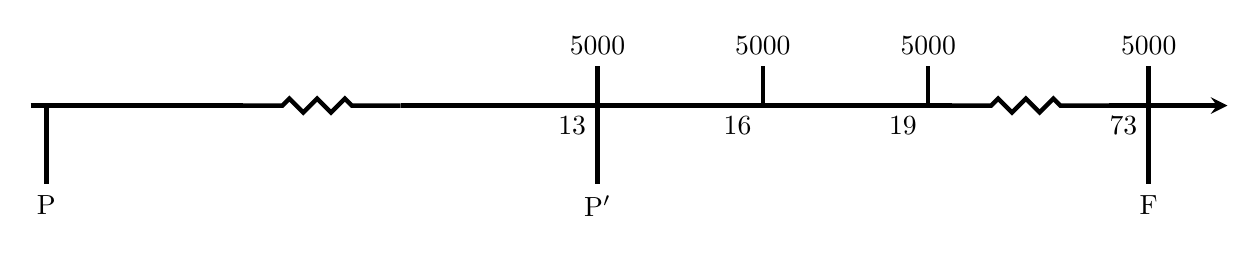
\begin{tikzpicture}[>=stealth,ultra thick]
    \draw[-] (-0.2,0) -- (2.5,0);
    \draw[decorate, decoration={zigzag,pre length=5mm, post length=5mm}][-] (2.5,0) -- (4.5,0);
    \draw[-] (4.5,0) -- (11.5,0);
    \draw[decorate, decoration={zigzag,pre length=5mm, post length=5mm}][-] (11.5,0) -- (13.5,0);
    \draw[->] (13.5,0) -- (15,0);
    \foreach \x/\n in {7/13,9.1/16,11.2/19,14/73}
      \draw (\x,0) node(\n)[below left] {\n} -- (\x,0.5);
    \foreach \x in {7,9.1,11.2,14}
      \draw (\x,0.5) node[above] {\num{5000}};
    \draw[-] (0,0) -- (0,-1);
    \draw (0,-1) node[below] {P};
    \draw[-] (7,0) -- (7,-1);
    \draw (7,-1) node[below] {P$^{\prime}$};
    \draw[-] (14,0) -- (14,-1);
    \draw (14,-1) node[below] {F};
  \end{tikzpicture}
  \begin{align*}
  A_E &= \frac{E({1.06}^3)}{(1.06 + {1.06}^2 + {1.06}^3)}\\
  &= 1764.67
  \end{align*}
  \begin{align*}
  F &= A\bigg(\frac{{(1+i)}^n - 1}{i}\bigg) &\vspace{40pt} P &= F{(1+i)}^{-n}\\
  &= 1764.67\bigg(\frac{{1.06}^{60} - 1}{0.06}\bigg) & &= 940795.31{(1.06)}^{-73}\\
  &= 940795.31 & &= 13371.10
  \end{align*}
  The present worth is \hilight{\$13,371.10}.
\end{itemize}
\end{document}
